  \subsection{Ejercicio 7}

  Para estudiar la performance del Round-Robin variando los cuantos creamos el lote7 y realizamos varias simulaciones. Variamos los quantums entre 1 y 10 inclusive y evaluamos el throughput y fairness con 2 y 4 n\'ucleos. Como las tareas TaskConsola son pseudoaleatorias,
  para cada selecci\'on de par\'ametros corrimos 10 simulaciones y graficamos el promedio con la variaci\'on estandard.

  \begin{figure}
  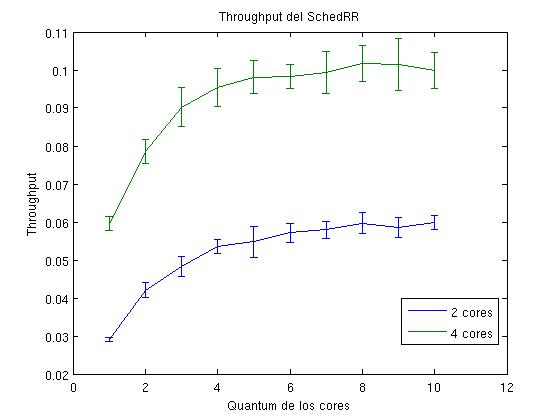
\includegraphics[scale=0.6]{images/TH.jpg}
  \caption{Throughput para SchedRR con dos y cuatro n\'ucleos}
  \end{figure}

  En la figura 6 se muestran los resultados del throughput. El throughput fue medido como $\frac{n}{T}$ con $n = $ cantidad de procesos y $T = $ tiempo de ejecuci\'on total. En la figura se observa que (considerando las desviaciones) el throughput aumenta al aumentar el quantum, tanto para 2 como 4 n\'ucleos. Esto tiene mucho sentido, ya que se
  gasta menos tiempo en cambios de contexto y es menos probable que un proceso cambie de CPU, bajando el costo total de migraci\'on de procesos entre CPUs. Obviamente, este crecimiento converge, ya que el tiempo que tardan en terminar los procesos est\'a acotado por
  el uso total del CPU dividido la cantidad de n\'ucleos, por lo que el throughput tambi\'en converge.

  \begin{figure}
  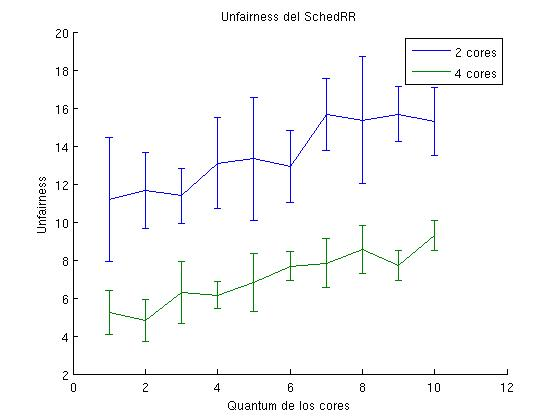
\includegraphics[scale=0.6]{images/fair.jpg}
  \caption{Throughput para SchedRR con dos y cuatro n\'ucleos}
  \end{figure}
  
  En la figura 7 se muestran los resultados de la fairness. La unfairness fue medida como la desviaci\'on standard de los waiting times, donde el waiting time es el tiempo de finalizaci\'on de ejecuci\'on menos el uso del CPU (para cada tarea).
  Esto tiene sentido ya que si la desviaci\'on estandard de los waiting times es chica entonces las tareas tienen waiting times similares, por lo que tienen usos de los n\'ucleos similares, lo que consituye un uso considerado fair.
  Por el contrario, si la desviaci\'on es alta se considera unfair. A pesar de las grandes variaciones, se observa a grandes rasgos que la unfairness tiende a aumentar con el tama\~no de los quantums. De la misma manera,
  la fairness disminuye con el tama\~no de los quantums. Esto es en gran medida esperable, ya que si hay quantums grandes es probable que haya tareas ejecutandose por mucho tiempo y que terminen de ejecutarse antes que otras hayan usado
  mucho procesamiento, incrementando las diferencias entre los waiting times.